\documentclass[a4paper,12pt,twoside]{memoir}

% Castellano
\usepackage[spanish,es-tabla]{babel}
\selectlanguage{spanish}
\usepackage[utf8]{inputenc}
\usepackage[T1]{fontenc}
\usepackage{lmodern} % scalable font
\usepackage{microtype}
\usepackage{placeins}

\RequirePackage{booktabs}
\RequirePackage[table]{xcolor}
\RequirePackage{xtab}
\RequirePackage{multirow}

% Links
\PassOptionsToPackage{hyphens}{url}\usepackage[colorlinks]{hyperref}
\hypersetup{
	allcolors = {red}
}

% Ecuaciones
\usepackage{amsmath}

% Rutas de fichero / paquete
\newcommand{\ruta}[1]{{\sffamily #1}}

% Párrafos
\nonzeroparskip

% Huérfanas y viudas
\widowpenalty100000
\clubpenalty100000

% Evitar solapes en el header
\nouppercaseheads


\let\tmp\oddsidemargin
\let\oddsidemargin\evensidemargin
\let\evensidemargin\tmp
\reversemarginpar



% Imagenes
\usepackage{graphicx}
\newcommand{\imagen}[2]{
	\begin{figure}[!h]
		\centering
		\includegraphics[width=0.9\textwidth]{#1}
		\caption{#2}\label{fig:#1}
	\end{figure}
	\FloatBarrier
}






\graphicspath{ {./img/} }

% Capítulos
\chapterstyle{bianchi}
\newcommand{\capitulo}[2]{
	\setcounter{chapter}{#1}
	\setcounter{section}{0}
	\setcounter{figure}{0}
	\setcounter{table}{0}
	\chapter*{#2}
	\addcontentsline{toc}{chapter}{#2}
	\markboth{#2}{#2}
}

% Apéndices
\renewcommand{\appendixname}{Apéndice}
\renewcommand*\cftappendixname{\appendixname}

\newcommand{\apendice}[1]{
	%\renewcommand{\thechapter}{A}
	\chapter{#1}
}

\renewcommand*\cftappendixname{\appendixname\ }

% Formato de portada
\makeatletter
\usepackage{xcolor}
\newcommand{\tutor}[1]{\def\@tutor{#1}}
%\newcommand{\tutorb}[1]{\def\@tutorb{#1}}
\newcommand{\course}[1]{\def\@course{#1}}
\definecolor{cpardoBox}{HTML}{E6E6FF}
\def\maketitle{
  \null
  \thispagestyle{empty}
  % Cabecera ----------------
\begin{center}
  \noindent
\includegraphics[width=\textwidth]{cabeceraSalud}\vspace{1.5cm}%
\end{center}
  
  % Título proyecto y escudo salud ----------------
  \begin{center}
    \begin{minipage}[c][1.5cm][c]{.20\textwidth}
        
\includegraphics[width=\textwidth]{escudoSalud.pdf}
    \end{minipage}
  \end{center}
  
  \begin{center}
    \colorbox{cpardoBox}{%
        \begin{minipage}{.8\textwidth}
          \vspace{.5cm}\Large
          \begin{center}
          \textbf{TFG del Grado en Ingeniería de la Salud}\vspace{.6cm}\\
          \textbf{\LARGE\@title{}}
          \end{center}
          \vspace{.2cm}
        \end{minipage}
    }%
  \end{center}
  
    % Datos de alumno, curso y tutores ------------------
  \begin{center}%
  {%
    \noindent\LARGE
    Presentado por \@author{}\\ 
    en Universidad de Burgos\\
    \vspace{0.5cm}
    \noindent\Large
    \@date{}\\
    \vspace{0.5cm}
    Tutor: \@tutor{}\\ % comenta el que no corresponda
    %Tutores: \@tutor{} -- \@tutorb{}\\
  }%
  \end{center}%
  \null
  \cleardoublepage
  }
\makeatother



% Datos de portada
\title{Seguimiento clínico de pacientes con afectaciones en
la mano con la ayuda de sensores de fuerza\\Documentación Técnica}
\author{Claudia Valentín Alguacil}
\tutor{Pedro Luis Sánchez Ortega}
%\tutorb{nombre tutor 2}
\date{\today}

\begin{document}

\maketitle



\cleardoublepage



%%%%%%%%%%%%%%%%%%%%%%%%%%%%%%%%%%%%%%%%%%%%%%%%%%%%%%%%%%%%%%%%%%%%%%%%%%%%%%%%%%%%%%%%



\frontmatter


\clearpage

% Indices
\tableofcontents

\clearpage

\listoffigures

\clearpage

\listoftables

\clearpage

\mainmatter

\appendix




\capitulo{1}{Planificación}
\section{Introducción}
Este anexo tiene como objetivo una presentación de manera integral de todos los aspectos clave relacionados con el desarrollo y la implementación del proyecto. 

Para realizar un correcto desarrollo del proyecto, se ha definido una planificación temporal y se desarrollará una planificación económica para saber el coste aproximado total del producto desarrollado.
\section{Planificación temporal}
El proyecto se ha desarrollado a lo largo de un total de 14 semanas(aproximadamente unos 4 meses), durante las cuales se ha distribuido el trabajo de forma progresiva. 

En la \textit{tabla \ref{fig:Planificación}} se puede observar una tabla donde se ha recogido la planificación temporal.
\begin{figure}[h]
        \centering
        \includegraphics[,width=0.5\textwidth]{img/planificacion.png}
        \caption{Planificación del proyecto}
        \label{fig:Planificación}
    \end{figure}

\section{Planificación económica}

La planificación económica consiste en el análisis total del precio del proyecto, incluyendo de manera individual los precios de los componentes del dispositivo (hardware), software y personal.

Todos los precios han sido obtenidos en 2025, por lo cual el coste puede variar en un futuro. 
\subsection{Precios Hardware}
Para calcular el precio total de los costes de los materiales del dispositivo, se tiene en cuenta la suma total de los precios de los componentes así como una suma de los gastos de producción y un porcentaje destinado a los beneficios. 

En la tabla \ref{tab:costes_hardware} se ha realizado un resumen de gastos y precio total. 
\begin{table}[]
\centering
\begin{tabular}{|l|p{8cm}|l|}
\hline
\rowcolor[HTML]{BFBFBF} 
\textbf{} & \textbf{Cálculos} & \textbf{Precio} \\ \hline
Gastos de los componentes & Suma total de los precios de los componentes del dispositvo & 60,37€\\ \hline
Gastos de producción & 10\% del precio de los
 componentes & 6,04€\\ \hline
Ingresos destinados a beneficio & 15\% de los gastos totales & 9,96€\\ \hline
\textbf{Total}& Suma total de los gastos & 76,37€ \\ \hline
\end{tabular}
\caption{Costes de dispositivos hardware.}
\label{tab:costes_hardware}
\end{table}

\subsubsection{\textbf{Desglose de precios de los componentes}}
Los precios de cada componente han sido seleccionados, siendo los mínimos encontrados en el mercado de páginas oficiales.
\begin{itemize}
    \item Placa Elegoo+USB: 15,99€
    \item Resistencias 5*0,01299€=0.064€
    \item Sensores de fuerza: 5*8,1€= 40,5€
    \item Elementos conectores(cables dupont): 14*0,07€=0.98€
    \item Protoboard=2,83€
\end{itemize}
No se han contemplado los gastos de la compra de un ordenador, ya que en la actualidad en toda área del hospital se cuenta con uno de forma habitual. 
\subsection{Precios software}

No se incluye ningún gasto en software ya que todo el material utilizado es gratuito y de código abierto.

\subsection{Precio de personal}
Para calcular el salario del personal se ha partido de los datos publicados de salarios de ingenieros biomédicos, profesionales con un perfil técnico y formativo parecido al ingeniero de la salud.
Actualmente, en España el sueldo medio de un ingeniero biomédico es de 3.500€ \cite{SueldoBioing}\footnote{Pagina web de indeed, donde se puede ver sueldos de diferentes trabajos  \cite{SueldoBioing}.}\cite{SUELDO}. Este sueldo es más bajo en recién egresados suponiendo un sueldo aproximado entre 1.500€ y 1.900€ mensuales.\cite{Sueldo_egresado}\footnote{Pagina web de la UAX con información económica sobre el salario de un graduado en ingeniería biomédica? \cite{Sueldo_egresado}.}.


En la tabla \ref{tab:costes_personal} se recoge el sueldo aproximado que debería cobrar por el proyecto un ingeniero de la salud.

\begin{table}[]
\centering
\begin{tabular}{|l|l|}
\hline
\rowcolor[HTML]{BFBFBF} 
\textbf{} & \textbf{Precio} \\ \hline
Sueldo mensual & 1.600€ \\ \hline
\textbf{Total en 4 meses }& 6.400€ \\ \hline
\end{tabular}
\caption{Costes de sueldos del personal.}
\label{tab:costes_personal}
\end{table}

\begin{table}[]
\centering
\begin{tabular}{|l|l|}
\hline
\rowcolor[HTML]{BFBFBF} 
\textbf{} & \textbf{Precio} \\ \hline
Material & 76,37€ \\ \hline
Sueldo  &  6.400€ \\ \hline
\textbf{Total }& 6.476,38€ \\ \hline
\end{tabular}
\caption{Precio total del proyecto}
\label{tab:Costes Totales}
\end{table}

\section{Viabilidad legal}
Se debe tener en cuenta la normativa legal desde la creación de la idea hasta la comercialización y uso postventa.

Es esencial la implementación de leyes que garanticen el cumplimiento de la normativa aplicable que respalde los derechos y obligaciones del autor.Incluyendo desde leyes de las regulaciones técnicas, de propiedad intelectual y de responsabilidad profesional, conforme a lo establecido en la legislación.

Asimismo, se debe implementar medidas vigorosas que protejan la integridad de los usuarios y la confidencialidad de sus datos. 

Podemos dividir el proceso en 2 fases, la primera fase incluiría la creación de la idea, diseño,desarrollo y realización de pruebas, y una segunda fase que incluya la comercialización y postventa.

\subsection{1º Fase}

Durante la primera fase de creación de la idea, diseño, desarrollo y realización de pruebas, se deberán incluir las siguientes normas legislativas: 

\begin{itemize}
    \item Ley 24/2015, de 24 de julio \cite{boe--2015-8328}, de Patentes: Establece los derechos, requisitos y procedimientos para obtener una patente y reforzar la seguridad jurídica.Esta ultima versión simplifica y agiliza el procedimiento.
    \item Real Decreto Legislativo 1/1996, de 12 de abril,\cite{boe--1996-8930} sobre la Ley de la Propiedad Intelectual: Establece los derechos de un obra al autor solo por el hecho de crearlo. 
    \item Real Decreto 192/2023, de 21 de marzo \cite{ministerio_de_sanidad_real_2023}, por el que se regulan los productos sanitarios. 
    \item UNE-EN 60601-1:2008 \cite{UNE2008}, norma que regula los requisitos generales para la seguridad básica y funcionamiento esencial de equipos electromédicos.
    \item UNE-EN ISO 14971:2020 \cite{UNE2020}, norma para la gestión de riesgos de dispositivos médicos.

\end{itemize}

\subsection{2º Fase}
Durante la segunda fase de comercialización y postventa, se deberán incluir las siguientes normas legislativas: 
\begin{itemize}
    \item Ley 3/1991, de 10 de enero \cite{boe--1991-628}, de Competencia Desleal, sobre la promoción y comercialización del producto,realizando una publicidad lícita, veraz y no engañosa.
    \item Ley Orgánica 3/2018, de 5 de diciembre \cite{boe--2018-16673}, de Protección de Datos Personales y garantía de los derechos digitales.
    \item Reglamento (UE) 2016/679 del Parlamento Europeo y del Consejo, de 27 de abril de 2016 \cite{boees}, relativo a la protección de las personas físicas en lo que respecta al tratamiento de datos personales y a la libre circulación de estos datos.
    \item Ley 29/2006, de 26 de julio \cite{boe--2006-13554}, de garantías y uso racional de los medicamentos y productos sanitarios.
\end{itemize}

\apendice{Documentación de usuario}
En esta sección del anexo se han definido aquellos requisitos necesarios para la ejecución y puesta en marcha del proyecto. 
\section{Requisitos software y hardware para ejecutar el proyecto.}
\subsection{Requisitos del software}
Para el correcto funcionamiento es necesario tener instalado en el ordenador todas las herramientas y programas que se han utilizado. 
\begin{itemize}
    \item Python: Este programa es esencial para que el código se ejecute y se abra el desplegable.
    \item Arduino IDE: Este programa es necesario para tener una comunicación y conexión correcta entre la placa de arduino y el ordenador 
    \item Editor de texto/codigo: No es estrictamente necesario la instalación de un editor de texto/codigo como Visual Estudio Code, pero si puede facilitar el uso tanto al usuario como a posibles profesionales ingenieros para la solución de errores.
    \item Instalación de bibliotecas:
    
    - Pandas: manipulación y analisis de datos estructurados(tablas)
    
    -Pyserial: comunicación con puerto serie
    
    -Kivy: paquete que permite la creación de la interfaz gráfica
    
    -kivymd: paquete que permite la creación de la interfaz gráfica

    -Openpyxl: abrir y modificar archivos excel.
    
    

\begin{table}[]
\centering
\begin{tabular}{|l|l|}
\hline
\rowcolor[HTML]{BFBFBF} 
\textbf{Software} & \textbf{Descripción} \\ \hline
Python & Versión 3.13\\ \hline
Arduino IDE & Versión 2.3.6\\ \hline
Bibliotecas & Versiones más actualizadas\\ \hline
\end{tabular}
\caption{Requisitos Software}
\label{tab:Requisitos_Software}
\end{table}
\end{itemize}
\subsection{Requisitos del hardware}
Para el correcto funcionamiento es necesario el uso del dispositivo creado, un ordenador y el cable USB que conecte el ordenador con la placa de Arduino.
\section{Instalación / Puesta en marcha}
\subsection{Python}

El proceso de descargar Python es sencillo. Desde la web oficial de Python \cite{Python}, en la pantalla inicial (ver figura \ref{fig:Python}), aparece un botón de descarga(señalado con una flecha roja). Al seleccionarlo, la descarga se inicia de forma  automática. Una vez descargado el archivo,el proceso de instalación se realiza de una forma similar a la de otras aplicaciones: se decide la ruta de instalación deseada y el programa queda instalado en nuestro ordenador.

\begin{figure}[h]
        \centering
        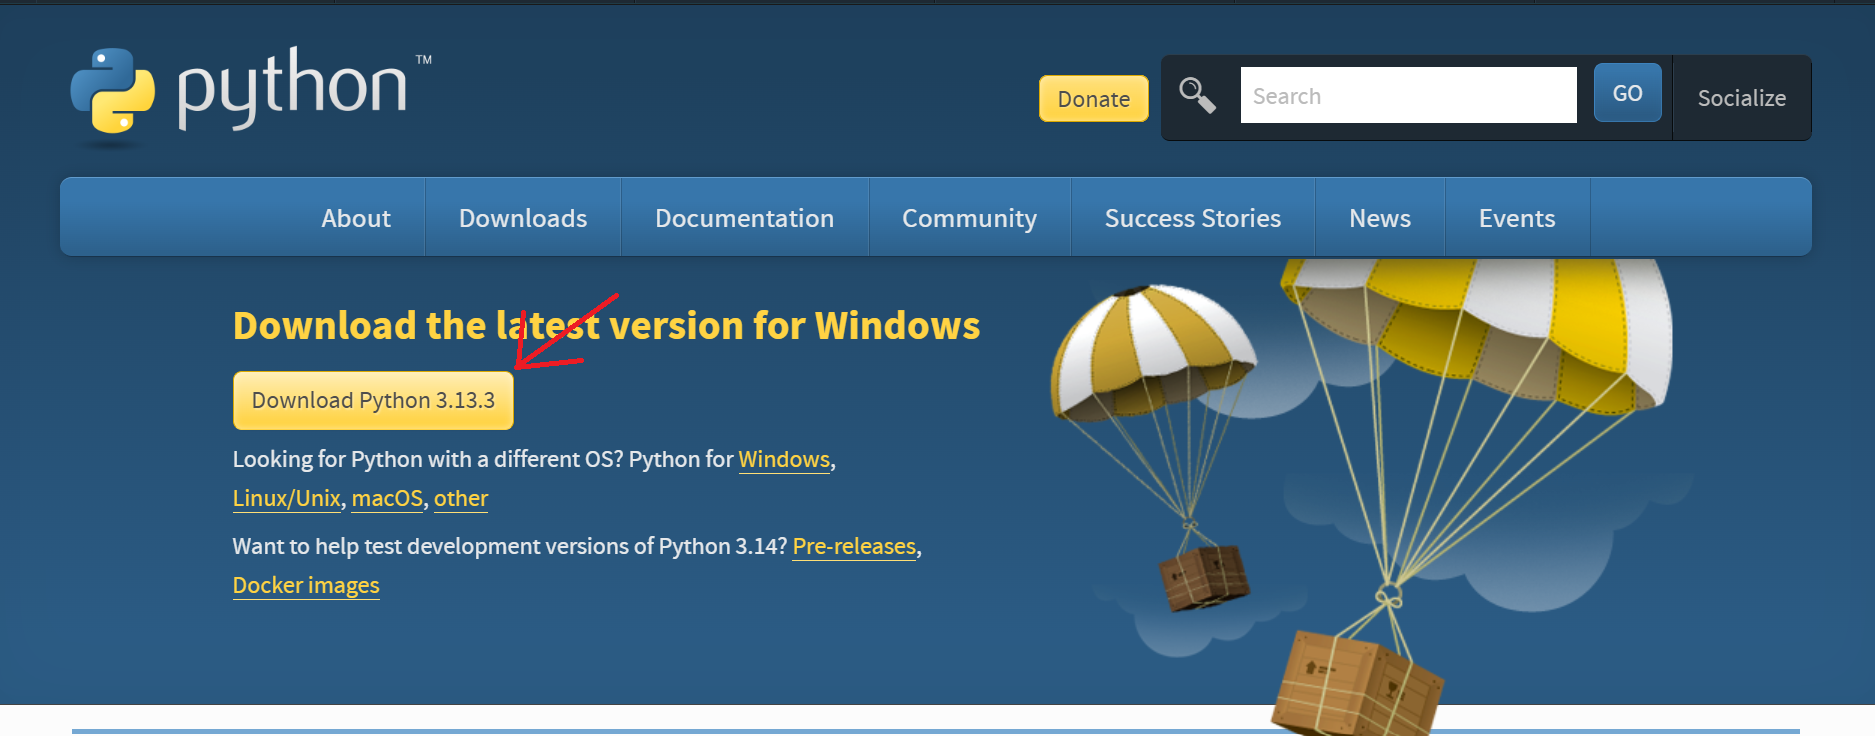
\includegraphics[width=0.8\textwidth]{img/pantalla inicio python.png}
        \caption{pantalla descargar Python}
        \label{fig:Python}
    \end{figure}
\subsection{Arduino IDE}
Proceso muy similar a la instalación de Python.Desde la web oficial de Arduino IDE \cite{Arduino}, en la pantalla inicial (ver figura \ref{fig:Arduino}), aparece una sección de diferentes opciones de descarga según el sistema operativo instalado en el ordenador. Al seleccionar el archivo correspondiente a nuestro sistema operativo, se abre una ventana nueva en la cual hay que clickear el botón 'Just Download' y la descarga se iniciará de forma  automática. Una vez descargado el archivo,el proceso de instalación se realiza de una forma similar a la de otras aplicaciones: se decide la ruta de instalación deseada y el programa queda instalado en nuestro ordenador.
    \begin{figure}[h]
        \centering
        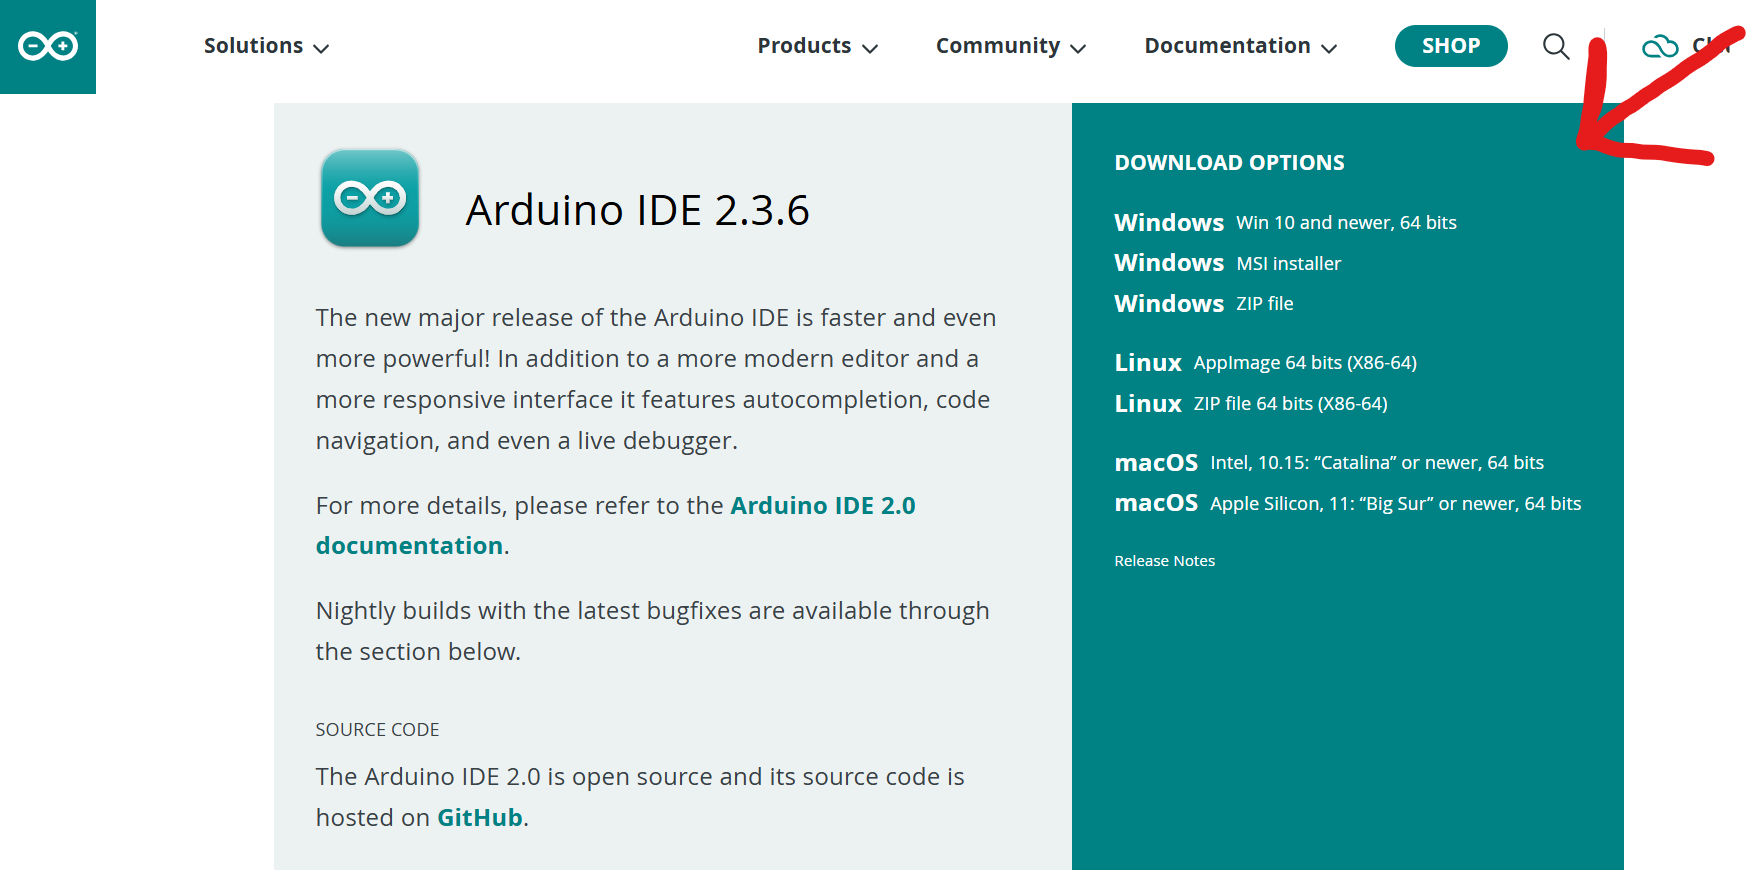
\includegraphics[width=1\textwidth]{img/pantalla inicio arduino IDE.png}
        \caption{pantalla descargar Arduino}
        \label{fig:Arduino}
    \end{figure}
\subsection{Instalación de bibliotecas}
La instalación de las bibliotecas se hace desde la consola del sistema (CMD).Para abrirla, basta con buscar CMD en el buscador de windows y hacer click sobre el resultado.
Una vez abierta la consola (ver figura\ref{fig:CMD}), se deben introducir los siguientes comandos para la instalación de las bibliotecas:

pip install pandas

pip intall pyserial

pip install kivy 

pip install kivymd

pip install openpyxl

\begin{figure}[h]
    \centering
    \includegraphics[width=0.8\textwidth]{img/pantalla CMD.png}
    \caption{pantalla CMD}
    \label{fig:CMD}
\end{figure}
\section{Manuales y/o Demostraciones prácticas}




    
     
\apendice{Manual del  programador.} 
\section{Estructura de directorios}
A continuación, se va a explicar la estructura de directorios situados en el Github.
\begin{itemize}
    \item AplicaciónEscritorio: Carpeta que contiene todo el código para la implementación de la interfaz.
    \begin{itemize}
        \item app.py: código de la interfaz
        \item interfaz.kv: código con el que se ha diseñado la interfaz
        \item Arduino.ino: Código arduino con el que se pueden realizar mediciones sin necesidad de la interfaz
    \end{itemize}
    \item Diseño: Carpeta que contiene el diseño del mango
    \item img: Carpeta que contiene todas las imágenes que se han utilizado para la realización del proyecto 
    \item tex:Carpeta que contiene todos los capítulos de la memoria y anexos
    \begin{itemize}
        \item 1\_introducción.tex: documento LaTeX en el que se realiza la descripción inicial del proyecto.
        \item 2\_objetivos.tex: documento LaTeX en el que se exponen  Objetivos principales del proyecto y personales.
        \item 3\_teoricos.tex: documento LaTeX que recoge los conceptos teóricos y el estado del arte.
        \item 4\_metodología.tex: documento LaTeX en el que se exponen las técnicas y herramientas utilizadas para la realización del proyecto.
        \item 5\_resultados.tex: documento LaTeX que recoge un resumen de los resultados del proyecto
        \item 6\_conclusión.tex: documento LaTeX en que se exponen las conclusiones que se han sacado en la realización del proyecto
        \item 7\_lineas\_futuras.tex: documento LaTeX que recoge las posibles lineas futuras que puede experimentar el proyecto.
        \item A\_planificación.tex: documento LaTeX en el que se expone la planificación temporal y economica y la viabilidad legal
        \item B\_manual\_usuario.tex: documento LaTeX que recogen aquellos requisitos necesarios para la ejecución y puesta en marcha del proyecto.
        \item C\_manual\_programador.tex: documento LaTeX que recoge la estructura de directioros del proyecto.
        \item D\_datos.tex: documento LaTeX que recoge la descripción de los datos recogidos.
        \item E\_diseño.tex: documento LaTeX que recoge los planos y el diseño del prototipo realizado.
        \item F\_requisitos.tex: documento LaTeX que incluye los casos de uso.
        \item G\_experimental.tex: documento LaTeX que detalla la configuración y parametrización de las técnicas utilizadas.
        \item H\_ODS.tex: documento LaTeX que incluye una reflexión personal sobre los aspectos de la sostenibilidad que se abordan en el proyecto.
    \end{itemize}
    \item Readme.md: archivo md (lenguaje de texto markdown) de presentación del proyecto en GitHub.
    \item Memoria\_Anexos\_PDF: Carpeta que contiene el documento de memoria y el de anexo en formato pdf.
    \begin{itemize}
        \item memoria.pdf: documento pdf con la memoria completa.
        \item anexo.pdf: documento pdf con el anexo completo.
    \end{itemize}
    \item anexo.tex:Documento LaTeX que contiene la estructura del anexo.
    \item memoria.tex: Documento LaTeX que contiene la estructura de la memoria.
    \item bibliografia.bib:Documento que recoge toda la bibliografía empleada en la memoria
    \item bibliografiaAnexos.bib:Documento que recoge toda la bibliografía empleada en el anexo
\end{itemize}
\section{Compilación, instalación y ejecución del proyecto}
Para la compilación y ejecución del proyecto es necesario: 
\begin{itemize}
    \item Instalación de Arduino IDE y Python
    \item Una vez instalados abrir la consola CMD e instalar las bibliotecas necesarias, especificadas en el apartado 2 del anexo B. 
    \item A continuación, será necesario la descarga de los archivos de la carpeta AplicacionEscritorio del repositorio de GitHub. Abrir el archivo Arduino.ino en la aplicación Arduino IDE, conectar la placa arduino mediante el puerto USB al ordenador y enviar el archivo a la placa. 
    \item Para finalizar, abrir el CMD o una aplicación de editor de texto como Visual Estudio Code, navegar hasta la localización de la carpeta y ejecutar python app.py 
\end{itemize}
\section{Instrucciones para la modificación o mejora del proyecto.}

\apendice{Descripción de adquisición y tratamiento de datos}

Como se ha especificado en la memoria, en el proyecto no se utilizan datos de fuentes externas, todos los datos son de elaboración propia.

Se pueden encontrar dos tipos de datos:
\begin{itemize}
    \item Proporcionados por el Usuario:
    \begin{itemize}
        \item Nombre del profesional. 
        \item Apellidos del profesional
        \item Contraseña para acceder al área.
        \item Nombre del paciente.
        \item Apellidos del paciente.
    \end{itemize}
        \item Datos recolectados por el dispositivo.
        \begin{itemize}
            \item Fecha y hora de cada medición.
            \item Los valores de fuerza/presión que ejerce cada dedo durante la medición:
            \begin{itemize}
                \item Pulgar en Kg
                \item Indice en Kg
                \item Corazón en Kg
                \item Anular en Kg
                \item Meñique en Kg
            \end{itemize}
        \end{itemize}
\end{itemize}
\include{./tex/E_diseno}
\apendice{Especificación de Requisitos}

\section{Diagrama de casos de uso}
En la figura \ref{fig:Diagrama Casos de uso} , se puede observar el diagrama de casos de uso definido para el uso del dispositivo. 

Existen 3 personas diferentes, ingeniero , usuario (sanitario) y el paciente, con funciones diferentes 
\begin{figure}
    \centering
    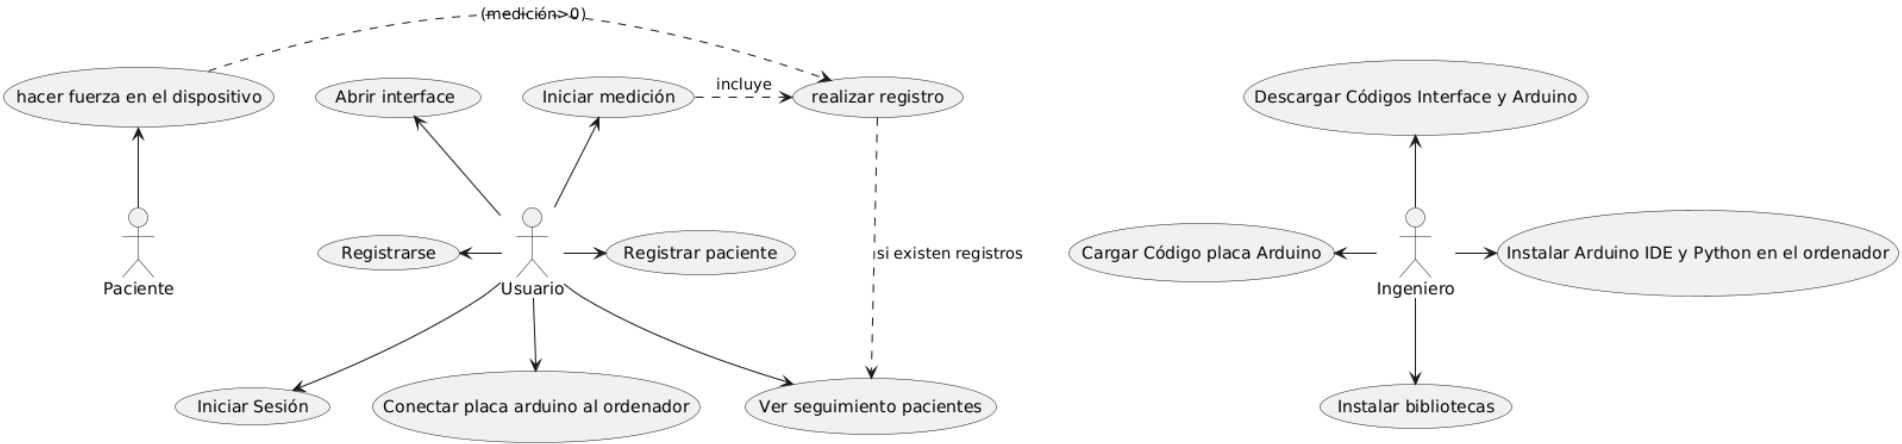
\includegraphics[width=1\linewidth]{img/Diagrama Casos de Uso.png}
    \caption{Diagrama Casos de uso. Fuente propia}
    \label{fig:Diagrama Casos de uso}
\end{figure}
\section{Explicación casos de uso.}

En esta sección se van a explicar de forma detallada cada uno de los casos de uso que se realizan, desde la puesta en marcha del dispositivo por los ingenieros hasta su uso en el hospital por los sanitarios.

\begin{table}[p]
	\centering
	\begin{tabularx}{\linewidth}{ p{0.21\columnwidth} p{0.71\columnwidth} }
		\toprule
		\textbf{CU-1}    & \textbf{Instalar Arduino IDE y Python}\\
		\toprule
		\textbf{Versión}              & 1.0    \\
		\textbf{Autor}                & Claudia Valentín Alguacil \\
		\textbf{Requisitos asociados} & RF-xx, RF-xx \\
		\textbf{Descripción}          & Instalación de ambas apps en el ordenador \\
		\textbf{Precondición}         & Tener acceso al ordenador del profesional \\
		\textbf{Acciones}             &
		\begin{enumerate}
			\def\labelenumi{\arabic{enumi}.}
			\tightlist
			\item Acceder a la web de ambas apps.
			\item Descargarlas en el ordenador.
                \item Instalarlas en el ordenador.
		\end{enumerate}\\
		\textbf{Postcondición}        &  Se podrán abrir ambas apps y ver el código \\
		\textbf{Excepciones}          & Sin acceso a internet no se pueden descargar. \\
		\textbf{Importancia}          & Alta \\
		\bottomrule
	\end{tabularx}
	\caption{CU-1 Nombre del caso de uso.}
\end{table}

\begin{table}[p]
	\centering
	\begin{tabularx}{\linewidth}{ p{0.21\columnwidth} p{0.71\columnwidth} }
		\toprule
		\textbf{CU-2}    & \textbf{Cargar código en la placa Arduino }\\
		\toprule
		\textbf{Versión}              & 1.0    \\
		\textbf{Autor}                & Claudia Valentín Alguacil \\
		\textbf{Requisitos asociados} & RF-xx, RF-xx \\
		\textbf{Descripción}          & Cargar código que produce que los sensores midan la fuerza generada por el paciente  \\
		\textbf{Precondición}         & Tener descargado e instalado Arduino IDE \\
		\textbf{Acciones}             &
		\begin{enumerate}
			\def\labelenumi{\arabic{enumi}.}
			\tightlist
			\item Abrir código Arduino.ino en Arduino IDE.
			\item Conectar placa arduino al ordenador mediante el cable USB.
                \item Mandar el código desde la aplicación a la placa Arduino.
		\end{enumerate}\\
		\textbf{Postcondición}        &  Se puede medir pesos\\
		\textbf{Excepciones}          & Conectar mal la placa o cable USB roto. \\
		\textbf{Importancia}          & Alta \\
		\bottomrule
	\end{tabularx}
	\caption{CU-2 Cargar código en la placa Arduino.}
\end{table}

\begin{table}[p]
	\centering
	\begin{tabularx}{\linewidth}{ p{0.21\columnwidth} p{0.71\columnwidth} }
		\toprule
		\textbf{CU-3}    & \textbf{Descargar códigos arduino e interfaz}\\
		\toprule
		\textbf{Versión}              & 1.0    \\
		\textbf{Autor}                & Claudia Valentín Alguacil \\
		\textbf{Requisitos asociados} & RF-xx, RF-xx \\
		\textbf{Descripción}          & Descargar los códigos que permiten utilizar el dispositivo y la interfaz \\
		\textbf{Precondición}         & Tener acceso a los códigos \\
		\textbf{Acciones}             &
		\begin{enumerate}
			\def\labelenumi{\arabic{enumi}.}
			\tightlist
			\item Acceder a la carpeta que contienen los archivos.
			\item Descargarlas en el ordenador.
		\end{enumerate}\\
		\textbf{Postcondición}        &  -- \\
		\textbf{Excepciones}          & Sin acceso a internet no se pueden descargar. \\
		\textbf{Importancia}          & Alta \\
		\bottomrule
	\end{tabularx}
	\caption{CU-3 Descargar los códigos que permiten utilizar el dispositivo y la interfaz}
\end{table}
% Caso de Uso 1 -> Consultar Experimentos.
\begin{table}[p]
	\centering
	\begin{tabularx}{\linewidth}{ p{0.21\columnwidth} p{0.71\columnwidth} }
		\toprule
		\textbf{CU-4} & \textbf{Instalar bibliotecas}\\
		\toprule
		\textbf{Versión}              & 1.0    \\
		\textbf{Autor}                & Claudia Valentín Alguacil \\
		\textbf{Requisitos asociados} & RF-xx, RF-xx \\
		\textbf{Descripción}          & Instalación de las bibliotecas necesarias para que el ordenador pueda procesar y abrir la interface sin problemas\\
		\textbf{Precondición}         & Tener descargado python en el ordenador \\
		\textbf{Acciones}             &
		\begin{enumerate}
			\def\labelenumi{\arabic{enumi}.}
			\tightlist
			\item Acceder al CMD del ordenador.
			\item Instalar una a una las bibliotecas.
		\end{enumerate}\\
		\textbf{Postcondición}        &  Se podrán abrir la interface sin ningun problema \\
		\textbf{Excepciones}          & Si no se instalan correctamente, no se podrá abrir la interfaz \\
		\textbf{Importancia}          & Alta \\
		\bottomrule
	\end{tabularx}
	\caption{CU-4 Instalar bibliotecas.}
\end{table}

\begin{table}[p]
	\centering
	\begin{tabularx}{\linewidth}{ p{0.21\columnwidth} p{0.71\columnwidth} }
		\toprule
		\textbf{CU-5}    & \textbf{Abrir interface}\\
		\toprule
		\textbf{Versión}              & 1.0    \\
		\textbf{Autor}                & Claudia Valentín Alguacil \\
		\textbf{Requisitos asociados} & RF-xx, RF-xx \\
		\textbf{Descripción}          & Proceso de abrir la interface por parte del sanitario \\
		\textbf{Precondición}         & Que el ingeniero haya realizado correctamente sus funciones de descarga e instalación de los diferentes paquetes y aplicaciones requeridas \\
		\textbf{Acciones}             &
        Opcion 1: 
		\begin{enumerate}
			\def\labelenumi{\arabic{enumi}.}
			\tightlist
			\item Abrir el CMD del ordenador.
			\item Navegar hasta la carpeta en la que esta el código descargado.
                \item Ejecutar el comando:
                
                \$ python app.py
		\end{enumerate}
        Opcion dos:
        \begin{itemize}
        \def\labelenumi{\arabic{enumi}.}
		  \tightlist
            \item Abrir Visual Estudio Code
            \item Abrir la carpeta donde se encuentra el codigo descargado.
            \item Ejecutar el comando:
                
            \$ python app.py
        \end{itemize} \\
		\textbf{Postcondición}        &  Se abre la interfaz. \\
		\textbf{Excepciones}          & Que haya algún fallo durante el proceso que realiza el ingeniero o que se acceda mal a la carpeta lo que produciría un error y no se desplegaría la interfaz \\
		\textbf{Importancia}          & Alta \\
		\bottomrule
	\end{tabularx}
	\caption{CU-6 Abrir interface.}
\end{table}

\begin{table}[p]
	\centering
	\begin{tabularx}{\linewidth}{ p{0.21\columnwidth} p{0.71\columnwidth} }
		\toprule
		\textbf{CU-7}    & \textbf{Registrarse}\\
		\toprule
		\textbf{Versión}              & 1.0    \\
		\textbf{Autor}                & Claudia Valentín Alguacil \\
		\textbf{Requisitos asociados} & RF-xx, RF-xx \\
		\textbf{Descripción}          & El sanitario se crea una cuenta en la interfaz para que pueda acceder en otras ocasiones. Este proceso produce una recopilación de datos personales como son el nombre, apellidos, nombre de usuario y  una contraseña  \\
		\textbf{Precondición}         & Que la interfaz abra correctamente y no tener un usuario ya registrado \\
		\textbf{Acciones}             &
		\begin{enumerate}
			\def\labelenumi{\arabic{enumi}.}
			\tightlist
			\item Abrir interfaz.
			\item Seleccionar botón de 'Registrarse'.
                \item Rellenar todos los datos requeridos.
                \item Seleccionar botón de 'Registrarse'.
		\end{enumerate}\\
		\textbf{Postcondición}        &  Usuario registrado lo que permitiría acceder a la siguiente pantalla iniciando sesión \\
		\textbf{Excepciones}          & Realizar mal el proceso de registro \\
		\textbf{Importancia}          & Media \\
		\bottomrule
	\end{tabularx}
	\caption{CU-7 Nombre del caso de uso.}
\end{table}

\begin{table}[p]
	\centering
	\begin{tabularx}{\linewidth}{ p{0.21\columnwidth} p{0.71\columnwidth} }
		\toprule
		\textbf{CU-8}    & \textbf{Iniciar sesión }\\
		\toprule
		\textbf{Versión}              & 1.0    \\
		\textbf{Autor}                & Claudia Valentín Alguacil \\
		\textbf{Requisitos asociados} & RF-xx, RF-xx \\
		\textbf{Descripción}          & El sanitario inicia sesión en la interfaz lo que permite que pueda visualizar los registros de sus pacientes, registrar nuevas cuantificaciones o pacientes. \\
		\textbf{Precondición}         & Tener una cuenta creada mediante el registro de nuevo usuario \\
		\textbf{Acciones}             &
		\begin{enumerate}
			\def\labelenumi{\arabic{enumi}.}
			\tightlist
                \item Abrir interfaz.
			\item Seleccionar botón de 'Iniciar sesión'.
                \item Rellenar la información de inicio de           sesión (usuario y contraseña).
                \item Seleccionar botón de 'Iniciar sesión'.
			\item La interfaz verifica la información recibida.
                \item Se accede a otra pantalla donde se puede visualizar los registros de sus pacientes,registrar nuevas cuantificaciones o pacientes.
		\end{enumerate}\\
		\textbf{Postcondición}    &  Acceder a la siguiente pantalla de la interfaz\\
		\textbf{Excepciones}  & Poner mal el usuario o contraseña. \\
		\textbf{Importancia} & Alta \\
		\bottomrule
	\end{tabularx}
	\caption{CU-8 Iniciar sesión .}
\end{table}

\begin{table}[p]
	\centering
	\begin{tabularx}{\linewidth}{ p{0.21\columnwidth} p{0.71\columnwidth} }
		\toprule
		\textbf{CU-9}    & \textbf{Registrar paciente.}\\
		\toprule
		\textbf{Versión}              & 1.0    \\
		\textbf{Autor}                & Claudia Valentín Alguacil \\
		\textbf{Requisitos asociados} & RF-xx, RF-xx \\
		\textbf{Descripción}          & Registrar el paciente en la interfaz, supone una recolección de datos como su nombre y apellidos que se recogerán en una base de datos \\
		\textbf{Precondición}  & Que no este el paciente ya registrado y que el sanitario haya iniciado sesión.\\
		\textbf{Acciones}             &
		\begin{enumerate}
			\def\labelenumi{\arabic{enumi}.}
			\tightlist
                \item Seleccionar botón de 'Registrar paciente'.
                \item Rellenar la información de registro del paciente (nombre y apellidos).
                \item Seleccionar botón de 'Registrar paciente'.
		\end{enumerate}\\
		\textbf{Postcondición} &  Se podrán registrar datos del usuario. \\
		\textbf{Excepciones} & -- \\
		\textbf{Importancia}          & Alta \\
		\bottomrule
	\end{tabularx}
	\caption{CU-9 Registrar paciente.}
\end{table}



\begin{table}[p]
	\centering
	\begin{tabularx}{\linewidth}{ p{0.21\columnwidth} p{0.71\columnwidth} }
		\toprule
		\textbf{CU-10}    & \textbf{Conectar la placa de arduino al ordenador.}\\
		\toprule
		\textbf{Versión}              & 1.0    \\
		\textbf{Autor}                & Claudia Valentín Alguacil \\
		\textbf{Requisitos asociados} & RF-xx, RF-xx \\
		\textbf{Descripción}          & Conectar el cable USB de la placa de arduino al puerto USB del ordenador \\
		\textbf{Precondición} & Tener el dispositivo(placa de arduino y sensores) \\
		\textbf{Acciones}             &
		\begin{enumerate}
			\def\labelenumi{\arabic{enumi}.}
			\tightlist
			\item Conectar cable USB al puerto USB del ordenador.
		\end{enumerate}\\
		\textbf{Postcondición}        &  Se podrá realizar la cuantificación de la presión ejercida \\
		\textbf{Excepciones}          & Conectar mal el USB \\
		\textbf{Importancia}          & Alta \\
		\bottomrule
	\end{tabularx}
	\caption{CU-10 Conectar la placa de arduino al ordenador.}
\end{table}

\begin{table}[p]
	\centering
	\begin{tabularx}{\linewidth}{ p{0.21\columnwidth} p{0.71\columnwidth} }
		\toprule
		\textbf{CU-11}    & \textbf{Iniciar medición}\\
		\toprule
		\textbf{Versión}              & 1.0    \\
		\textbf{Autor}                & Claudia Valentín Alguacil \\
		\textbf{Requisitos asociados} & RF-xx, RF-xx \\
		\textbf{Descripción}          & Proceso de cuantificar los valores que recoge los sensores. \\
		\textbf{Precondición}         & Conectar placa de arduino al ordenador y tener desplegado la interfaz. \\
		\textbf{Acciones}             &
		\begin{enumerate}
			\def\labelenumi{\arabic{enumi}.}
			\tightlist
			\item Seleccionar al paciente con el que se quiera registrar una nueva cuantificación.
			\item Conectar la placa de arduino al ordenador.
                \item Seleccionar botón iniciar medición de la interfaz y pulsar el pin botón del dispositivo.
		\end{enumerate}\\
		\textbf{Postcondición}        &  Ver seguimiento pacientes\\
		\textbf{Excepciones}          & No conectar la placa al ordenador. \\
		\textbf{Importancia}          & Media \\
		\bottomrule
	\end{tabularx}
	\caption{CU-11 Iniciar medición.}
\end{table}

\begin{table}[p]
	\centering
	\begin{tabularx}{\linewidth}{ p{0.21\columnwidth} p{0.71\columnwidth} }
		\toprule
		\textbf{CU-12}    & \textbf{Ejercer fuerza en los sensores}\\
		\toprule
		\textbf{Versión}              & 1.0    \\
		\textbf{Autor}                & Claudia Valentín Alguacil \\
		\textbf{Requisitos asociados} & RF-xx, RF-xx \\
		\textbf{Descripción}          & El paciente debe de realizar fuerza en los sensores del dispositivo, colocando cada dedo según el sensor en el que corresponde. \\
		\textbf{Precondición}         &  Casos de Uso :09,11 y 12\\
		\textbf{Acciones}             &
		\begin{enumerate}
			\def\labelenumi{\arabic{enumi}.}
			\tightlist
			\item Conectar placa arduino al ordenador.
			\item Seleccionar iniciar medición.
                \item Hacer fuerza en la mano.
		\end{enumerate}\\
		\textbf{Postcondición}        &  Se podrá observar los datos recogidos en la tabla. \\
		\textbf{Excepciones}          & Mala captación de datos. \\
		\textbf{Importancia}          & Media \\
		\bottomrule
	\end{tabularx}
	\caption{CU-12 Hacer fuerza en el dispositivo.}
\end{table}

\begin{table}[p]
	\centering
	\begin{tabularx}{\linewidth}{ p{0.21\columnwidth} p{0.71\columnwidth} }
		\toprule
		\textbf{CU-13}    & \textbf{Ver seguimiento pacientes}\\
		\toprule
		\textbf{Versión}              & 1.0    \\
		\textbf{Autor}                & Claudia Valentín Alguacil \\
		\textbf{Requisitos asociados} & RF-xx, RF-xx \\
		\textbf{Descripción}          & Visualización de los registros de los pacientes realizadas mediante la cuantificación de la presión/fuerza que se ejerce a los sensores.\\
		\textbf{Precondición}         & Tener registros \\
		\textbf{Acciones}             &
		\begin{enumerate}
			\def\labelenumi{\arabic{enumi}.}
			\tightlist
			\item Acceder a la pantalla del paciente del que queramos observar el seguimiento.
			\item Seleccionar 'Visualización Registro'.
                \item Visualizar todos los registros realizados.
		\end{enumerate}\\
		\textbf{Postcondición}        &  -- \\
		\textbf{Excepciones}          & -- \\
		\textbf{Importancia}          & Baja/Media \\
		\bottomrule
	\end{tabularx}
	\caption{CU-13 Ver seguimiento pacientes.}
\end{table}


\newpage

\section{Prototipos de interfaz o interacción con el proyecto.}

Se ha realizado un prototipo de interfaz para ordenador, tipo desplegable, en base a las necesidades y requisitos para su uso. 

Esta interfaz creada consta de 7 pantallas:
\begin{enumerate}
    \item Pantalla Principal: es la pantalla de presentación (véase figura \ref{fig:Pantalla principal}), en ella se muestra el logo de la aplicación , dos botones, iniciar sesión y registrarse, y un recuadro con información relevante sobre la interfaz.
    \begin{figure}
        \centering
        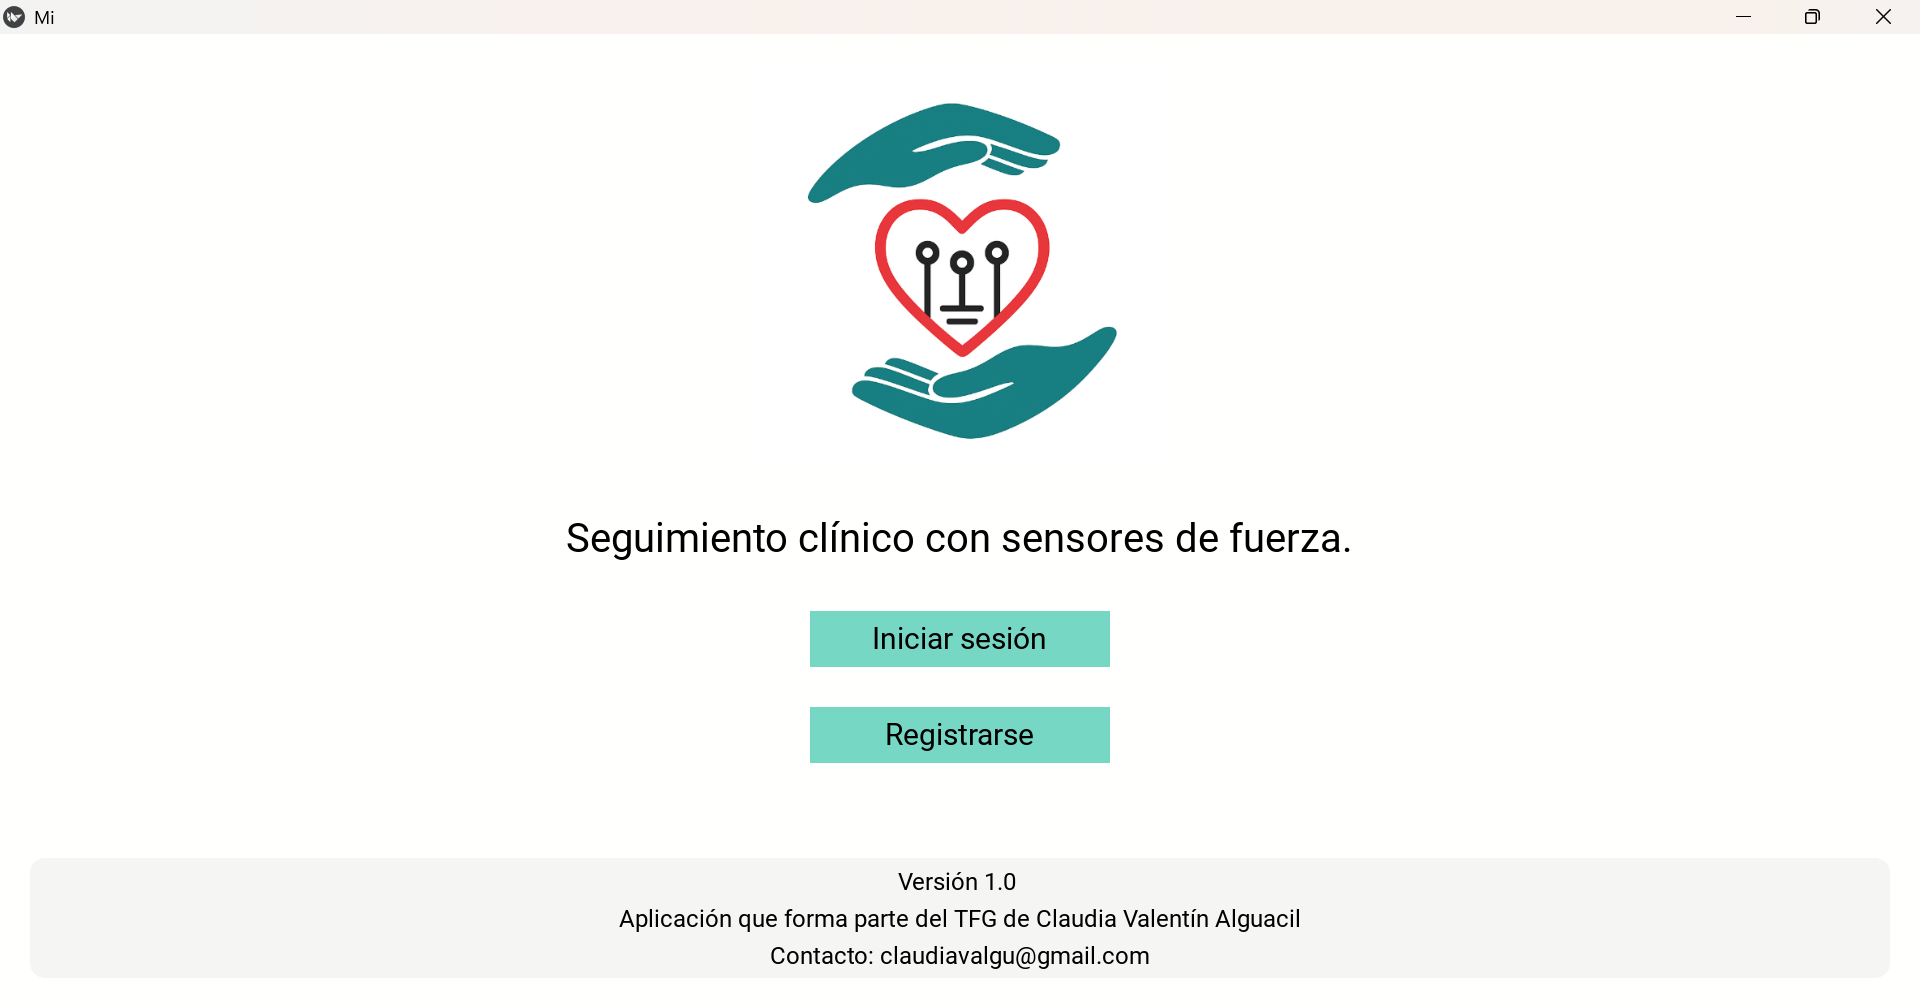
\includegraphics[width=1\linewidth]{img/Pantalla principal.png}
        \caption{Pantalla principal. Fuente Propia.}
        \label{fig:Pantalla principal}
    \end{figure}
    \item Pantalla Inicio Sesión: es la pantalla que permite al usuario (sanitario) iniciar sesión en la interfaz (véase figura \ref{fig:Pantalla Inicio Sesión}), en ella se debe introducir el usuario y contraseña personal de cada usuario para acceder al área. Desde esta pantalla, se puede volver a la pantalla principal seleccionando el botón 'Volver' o bien, acceder a la siguiente pantalla seleccionando el botón 'Entrar'.
\begin{figure}
    \centering
    \includegraphics[width=1\linewidth]{img/Pantalla Inicio Sesión.png}
    \caption{Pantalla Inicio Sesión.Fuente Propia.}
    \label{fig:Pantalla Inicio Sesión}
\end{figure}
    \item Pantalla Registrar Usuario: es la pantalla que permite al usuario (sanitario) registrarse en la interfaz (véase figura \ref{fig:img/Pantalla Registrar Usuario}), en ella se debe introducir el nombre, apellidos, nombre de usuario y contraseña personal. Estos datos se almacenarán en un documento Json.Desde esta pantalla, se puede volver a la pantalla principal sin registrar un nuevo usuario seleccionando el botón 'Volver' o bien, registrar un nuevo usuario seleccionando el botón 'Registrarse'. Realizando la ultima acción la app te dirige de forma automático a la pantalla principal
    \begin{figure}
        \centering
        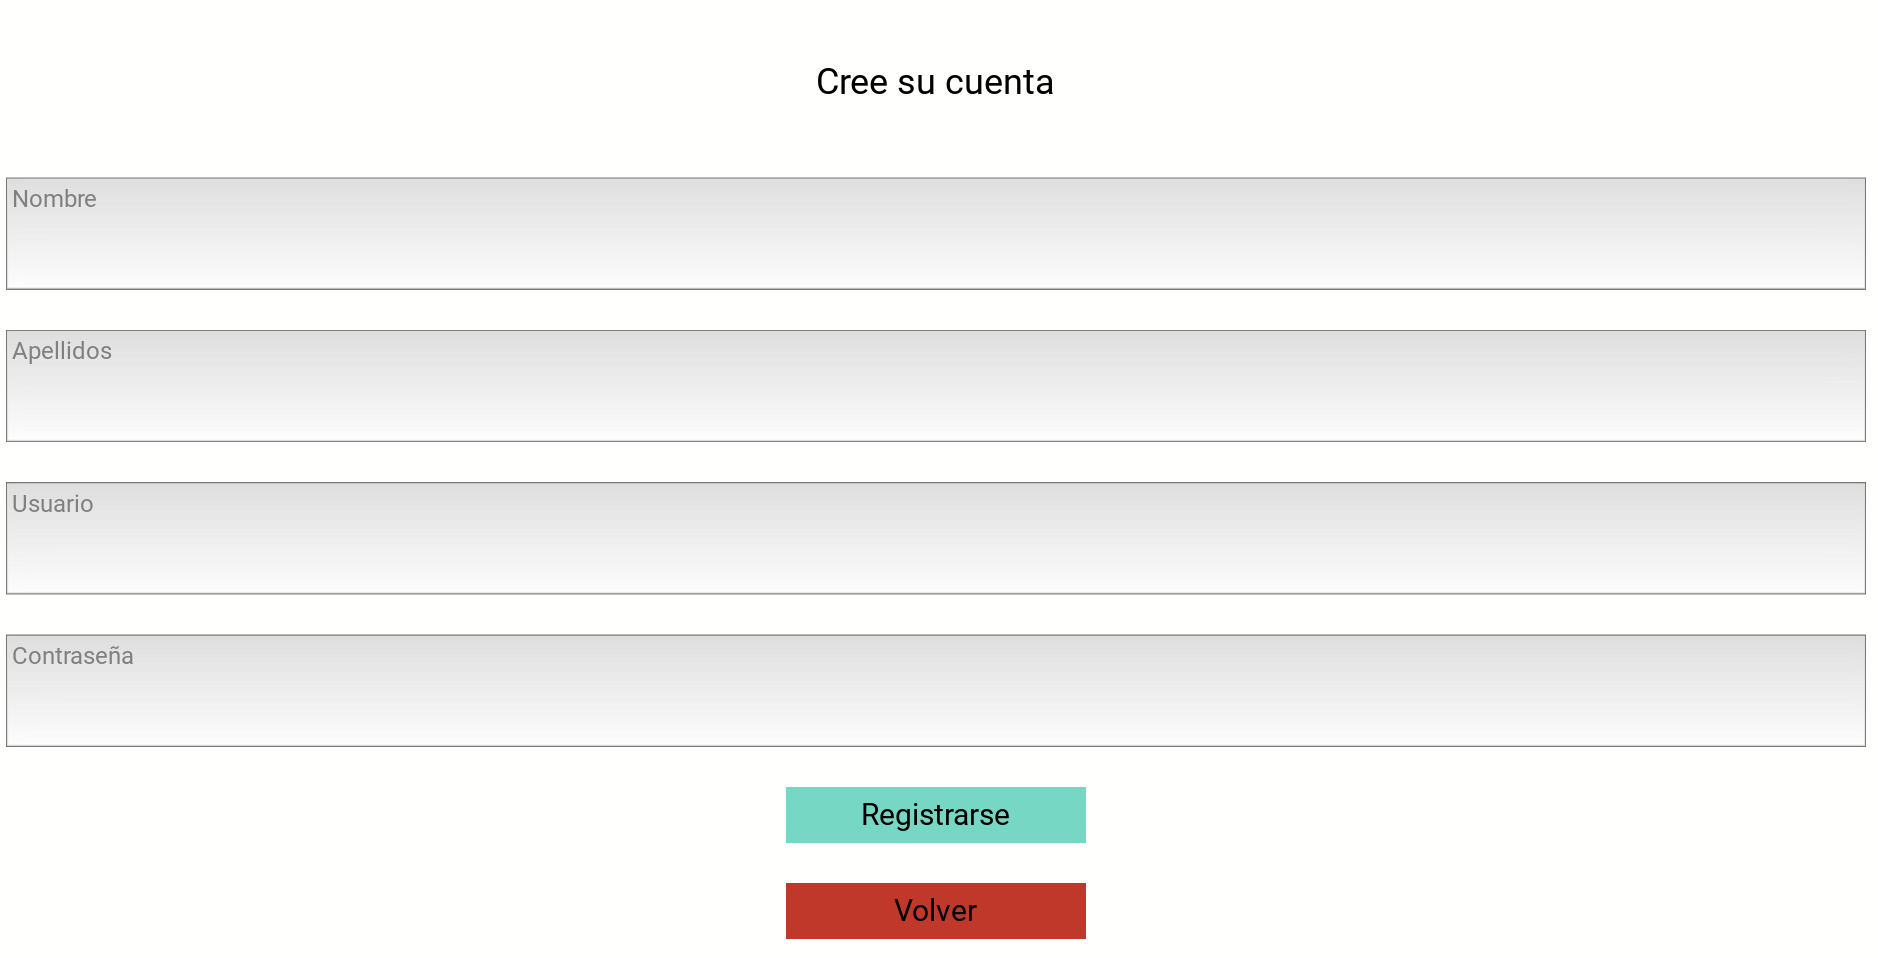
\includegraphics[width=1\linewidth]{img/Pantalla Registrar Usuario.png}
        \caption{img/Pantalla Registrar Usuario.Fuente propia}
        \label{fig:img/Pantalla Registrar Usuario}
    \end{figure}
    \item Pantalla de Inicio: es la pantalla principal de cada usuario (véase figura\ref{fig:Pantalla Inicio} ). Consta de un recuadro con el nombre y apellidos del profesional, un mensaje de bienvenida y dos botones, uno de seleccionar paciente y otro de registrar paciente. Si seleccionamos el primero de ellos, sale un menú desplegable con los diferentes nombre y apellidos de los pacientes registrados. Si seleccionamos el segundo botón, nos dirige a una pantalla nueva que nos permitirá el registro de un nuevo paciente.
    \begin{figure}
        \centering
        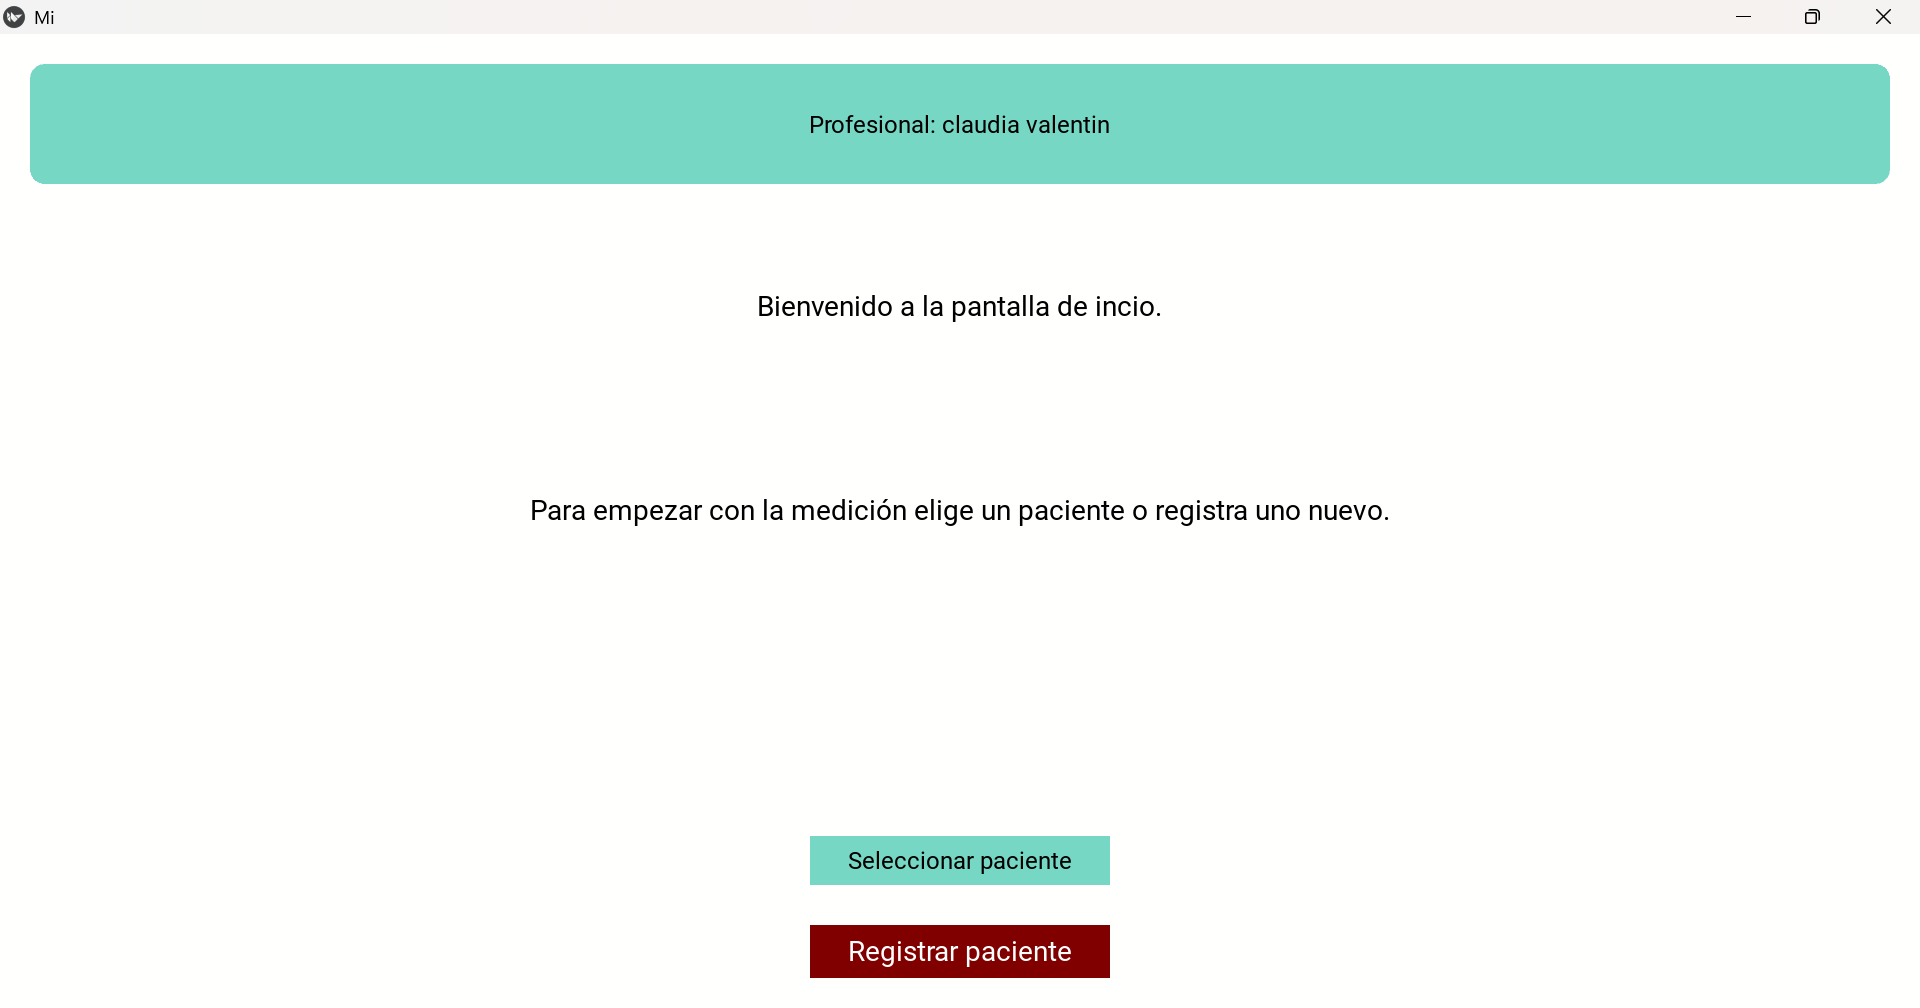
\includegraphics[width=1\linewidth]{img/Pantalla Inicio.png}
        \caption{Pantalla Inicio. Fuente Propia}
        \label{fig:Pantalla Inicio}
    \end{figure}
\end{enumerate}
\apendice{Estudio experimental}
Durante la realización del proyecto, no se ha realizado un estudio experimental. 

La realización de este seria esencial en un futuro cuando se haya obtenido un dispositivo final antes de lanzarlo al mercado. 

Sería útil realizar un estudio con un conjunto de pacientes para hacer un seguimiento de los datos recogidos por el dispositivo y observar cómo evolucionan desde la primera sesión hasta que finalmente se les da de alta.
De esta manera, se podría observar si las sesiones están resultado positivas o, en caso contrario, determinar si deberían interrumpirse para que un nuevo paciente en lista de espera pueda acceder a las sesiones de terapia.

\section{Configuración y parametrización de las técnicas.}

Para una correcta cuantificación de la fuerza ejercida a los sensores se ha realizado una parametrización de los sensores de fuerza resistivos. 

Al emplear este tipo de sensores para medir, la relación entre el nivel de cuantificación y la magnitud del peso no se comporta de manera lineal, sino que la curva característica muestra un comportamiento exponencial o logarítmico. 

En este proceso, primero se ha hecho una relación entre 10 pesos y el valor leído por el sensor (véase tabla \ref{tab:Relación Valor-Peso}). 
\begin{table}[h]
    \centering
    \begin{tabular}{|c|c|}
    \rowcolor[HTML]{BFBFBF} 
        \hline
        \textbf{Valor} & \textbf{Peso (kg)} \\ \hline
        0   & 0    \\ \hline
        165 & 0,5  \\ \hline
        258 & 1    \\ \hline
        302 & 1,5  \\ \hline
        340 & 2    \\ \hline
        368 & 2,5  \\ \hline
        404 & 3    \\ \hline
        440 & 3,5  \\ \hline
        460 & 4    \\ \hline
        498 & 4,5  \\ \hline
   \end{tabular}
    \caption{Relación Valor-Peso}
    \label{tab:Relación Valor-Peso}
\end{table}
Dado que solo se han obtenido diez valores experimentales, los valores que se encuentren entre dos de estos se determinan mediante interpolación lineal, que sigue la siguiente fórmula:
\begin{equation}
    y = \frac{y_1 - y_0}{x_1 - x_0} \cdot (x - x_0) - y_0
    \label{eq: Interpolación lineal}
\end{equation}

Dado que utilizamos este tipo de ecuación, los resultados no son 100\% reales, pero sí aproximados.

En la figura \ref{fig:Grafica peso-valor} se puede observar cómo crece la curva que relaciona los valores medidos con los pesos. El crecimiento de los primeros valores es considerablemente más pronunciado en comparación con los valores obtenidos con pesos más altos, lo cual se debe al comportamiento característico de los sensores de fuerza resistivos. 
\begin{figure}
    \centering
    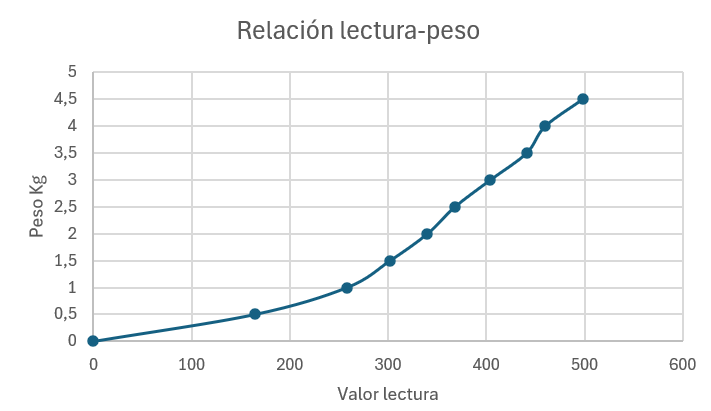
\includegraphics[width=0.75\linewidth]{img/Grafica peso-valor.png}
    \caption{Gráfica peso-valor. Fuente propia}
    \label{fig:Grafica peso-valor}
\end{figure}

Dado que al medir la fuerza ejercida se pueden crear picos máximos o mínimos falsos, se ha implementado la fórmula de la desviación estándar.
\begin{equation}
    \sigma=\sqrt{\frac{\sum\left(x_{i}-\mu\right)^{2}}{N}}
\end{equation}
Donde sigma es la desviación estándar, mu es la media, xi es cada valor muestreado y N es el total muestreado.
\apendice{Anexo de sostenibilización curricular}

El desarrollo sostenible es un conjunto de principios aprobados en 2015 por la Organización de las Naciones Unidas (ONU), y recogidos en la Agenda 2030. La Agenda 20230 para el Desarrollo Sostenible es un plan de acción a nivel global, actualmente respaldada por los 193 países que pertenecen a la ONU, a favor de las personas, el planeta y las prosperidad económica, sanitaria y social, que además aboga por la paz universal y el acceso a la justicia \cite{Agenda2030_gobierno}

El desarrollo sostenible es considerado una oportunidad de mejora en la calidad de vida de todos los ciudadanos, sin excluir a nadie. Esto implica, entre otros objetivos, erradicar la pobreza, poner fin a todas las guerras, fomentar el acceso a una educación de calidad, adecuada y universal, garantizar unos servicios sanitarios universales, eficaces y de calidad, promover ciudades y comunidades inclusivas, seguras, resilientes y sostenibles. Para cumplir con todos los objetivos requieren de la cooperación de instituciones y gobiernos que aseguren mediante leyes e impulsos el cumplimiento y colaboración por parte de la sociedad. \cite{ODS}

Cada uno de los 17 Objetivos de Desarrollo Sostenible (ODS), conlleva unas metas concretas cuyos fines deben alcanzarse antes del año 2030. En la \textit{Figura} \ref{fig:ODS}, se exponen cada uno de estos ODS.

\begin{figure}
    \centering
    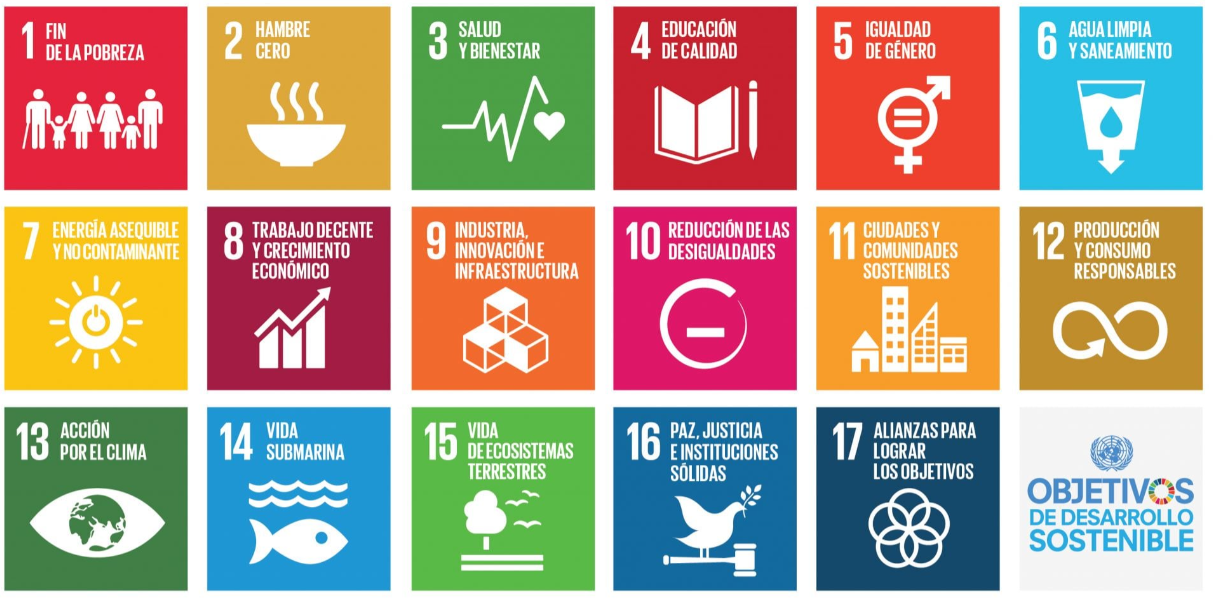
\includegraphics[width=1\linewidth]{img/ODS.png}
    \caption{17 ODS. Fuente un.org}
    \label{fig:ODS}
\end{figure}

Dentro del desarrollo de este proyecto, se han identificado tres ODS particularmente relacionados, ya que la creación de un dispositivo de medición de la fuerza de los dedos y seguimiento puede contribuir con los objetivos marcados en la Agenda 2030, no solo en términos tecnológicos, sino también sociales y sanitarios.

En primer lugar, el ODS 3: Salud y Bienestar, cobra especial relevancia. Este objetivo busca el acceso universal a servicios sanitarios, garantizar una vida sana y promover el máximo bienestar posible para todas las personas y en todos los rangos de edades. El dispositivo y aplicación desarrollados en este proyecto tiene como finalidad facilitar el seguimiento y evaluación de los pacientes en rehabilitación de la mano, proporcionando una herramienta especialmente útil en contextos clínicos y terapéuticos. Asimismo, su diseño desde el inicio se ha planteado con un enfoque versátil, accesible y de bajo coste, lo cual permite su implementación en distintos tipos de centros sanitarios, incluyendo aquellos con recursos limitados. De este modo, se promueve una atención sanitaria más equitativa, eficiente y adaptada a las necesidades individuales de cada paciente, favoreciendo la recuperación funcional. \cite{salud_ODS}

En segundo lugar, el proyecto se relaciona con el ODS 9: Industria, Innovación e Infraestructura, cuyo objetivo es construir infraestructuras resilientes, promover la industrialización sostenible y fomentar la innovación. La creación de un dispositivo médico funcional, accesible y basado en tecnologías emergentes representa una aportación directa a la innovación tecnológica aplicada a la salud. \cite{infraestructura_ODS}

Por último, el ODS 10: Reducción de las Desigualdades, también se ve reflejado en este proyecto. Este objetivo busca reducir la desigualdad en y entre los países, promoviendo y potenciando la inclusión social, económica y política de todas las personas, independientemente de su edad, género, condición física o situación económica. Los prototipos desarrollados pueden contribuir a la ampliación en el acceso a tecnologías de rehabilitación, permitiendo que personas con escasos recursos o con discapacidades físicas puedan beneficiarse de tratamientos más personalizados, medibles y eficaces. Además, la posibilidad de adaptabilidad del sistema permite su uso por parte un gran número de profesionales para usuarios con diferentes patologías, lo que lo hace especialmente útil.\cite{desigualdades_ODS}

En conclusión, la creación de estos prototipos supone una pequeña contribución al cumplimiento de los ODS. Proporcionando una nueva tecnología, que impulsa el crecimiento de la industria y ámbitos sanitarios, fomentando la inclusión y reduciendo desigualdades.



\bibliographystyle{apalike}
\bibliography{bibliografiaAnexos}

\end{document}